% This file was created with tikzplotlib v0.10.1.
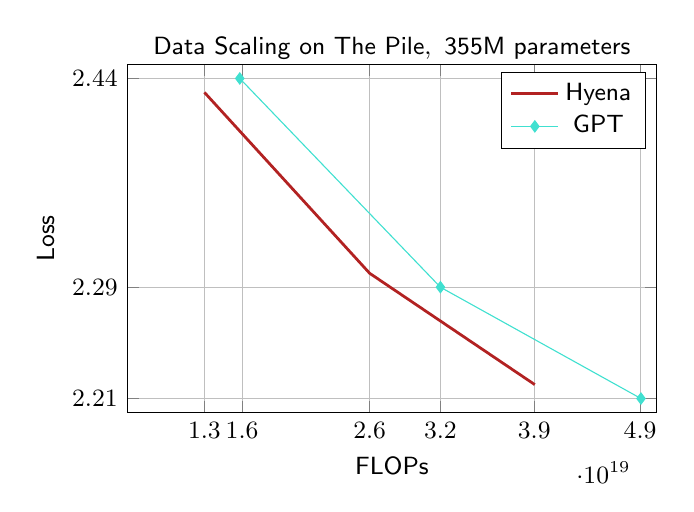
\begin{tikzpicture}[font=\small]

\definecolor{brown}{RGB}{165,42,42}
\definecolor{darkgray176}{RGB}{176,176,176}
\definecolor{firebrick}{RGB}{178,34,34}
\definecolor{indianred}{RGB}{205,92,92}
\definecolor{lightgray204}{RGB}{204,204,204}
\definecolor{lightseagreen}{RGB}{32,178,170}
\definecolor{teal}{RGB}{0,128,128}
\definecolor{turquoise}{RGB}{64,224,208}

\begin{axis}[
width=8.3cm, height=6cm,
title={$\small{{\sf Data~Scaling~on~The~Pile,~355M~parameters}}$},
title style = {at={(.5, .94)}},
xlabel={$\small \sf FLOPs$}, ylabel={$\small\sf Loss$}, 
ylabel style={at={(-.12,.5)}},
xmin=7e+18, xmax=4.9e+19, ymin=2.2, ymax=2.45,
major grid style={lightgray,thin},
minor grid style={lightgray,very thin},
grid=both,
%
xtick={1.311e+19,1.61e+19,2.623e+19,3.185e+19,3.93e+19,4.77e+19},
xticklabels={
  \(\displaystyle {1.3}\),
  \(\displaystyle {1.6}\),
  \(\displaystyle {2.6}\),
  \(\displaystyle {3.2}\),
  \(\displaystyle {3.9}\),
  \(\displaystyle {4.9}\)
},
ytick={2.44, 2.29, 2.21},
yticklabels={
  \(\displaystyle {2.44}\),
  \(\displaystyle {2.29}\),
  \(\displaystyle {2.21}\)
}
]
\addplot [mark=mystar, line width=1pt, firebrick]
table{%
x  y
1.311e+19 2.43
2.623e+19 2.30
3.934e+19 2.22
};\addlegendentry{$\sf Hyena$};
\addplot [draw=black, mark=diamond*, turquoise]
table{%
x  y
1.592e+19 2.44
3.185e+19 2.29
4.777e+19 2.21
};\addlegendentry{$\sf GPT$};
% \addplot [line width=1pt, indianred, opacity=0.4]
% table {%
% 3.227256e+18 17.01
% 6.454512e+18 14.16
% 9.681768e+18 12.58
% 1.2909024e+19 11.82
% 1.613628e+19 11.44
% };
% \addplot [line width=1pt, turquoise, opacity=0.4]
% table {%
% 4.12e+18 17.91
% 8.24e+18 14
% 1.236e+19 12.55
% 1.648e+19 11.76
% 2.06e+19 11.44
% };
% \addplot [line width=1pt, lightseagreen, opacity=0.4]
% table {%
% 4.12e+18 17.84
% 8.24e+18 13.92
% 1.236e+19 12.61
% 1.648e+19 11.62
% 2.06e+19 11.04
% 2.472e+19 10.59
% 2.884e+19 10.28
% 3.296e+19 10.04
% 3.708e+19 9.88
% 4.12e+19 9.79
% };
% \addplot [line width=1pt, teal, opacity=0.4]
% table {%
% 4.12e+18 17.76
% 8.24e+18 13.82
% 1.236e+19 12.43
% 1.648e+19 11.57
% 2.06e+19 11.04
% 2.472e+19 10.61
% 2.884e+19 10.27
% 3.296e+19 10.01
% 3.708e+19 9.79
% 4.12e+19 9.61
% 4.532e+19 9.55
% 4.944e+19 9.33
% 5.356e+19 9.23
% 5.768e+19 9.16
% 6.18e+19 9.12
% };
% \addplot [line width=1pt, brown, opacity=0.4]
% table {%
% 3.227256e+18 17.03
% 6.454512e+18 13.76
% 9.681768e+18 12.46
% 1.2909024e+19 11.67
% 1.613628e+19 11.2
% 1.9363536e+19 10.74
% 2.2590792e+19 10.37
% 2.5818048e+19 10.09
% 2.9045304e+19 9.9
% 3.227256e+19 9.8
% };
% \addplot [line width=1pt, firebrick, opacity=0.4]
% table {%
% 3.227256e+18 17.25
% 6.454512e+18 14.26
% 9.681768e+18 12.58
% 1.2909024e+19 11.95
% 1.613628e+19 11.46
% 1.9363536e+19 11.05
% 2.2590792e+19 10.72
% 2.5818048e+19 10.43
% 2.9045304e+19 10.18
% 3.227256e+19 9.97
% 3.5499816e+19 9.78
% 3.8727072e+19 9.62
% 4.1954328e+19 9.48
% 4.5181584e+19 9.35
% 4.840884e+19 9.24
% };
% % linear regressed values
% \addplot [line width=1pt, dotted, red, opacity=1]
% table {%
% 1.2e+19 11.54196759
% 7.2e+19 7.45180555
% };
% %
% \addplot [line width=1pt, dotted, blue, opacity=1]
% table {%
% 1.2e+19 11.76093851
% 7.2e+19 8.38229773
% };
\end{axis}

\end{tikzpicture}
